\chapter{Introduction}\label{chapter_introduction}
A central issue addressed in this dissertation is the possibility of recurrent behaviors discovery 
from publicly available software process artifacts. 

As recurrent behaviors are considered to be the basic building blocks of any human-driven
\textit{goal-oriented} process, which reflect the development of more or less fixed ways of dealing 
with tasks \textit{based on past performance} \cite{neal2012habits} \cite{1903}, 
then, the ability to discover recurrent behaviors in the context of software development equates 
to a highly desirable capacity to discover the evolution of characteristic mannerisms in which developers 
structure their activities -- the antecedent features that form high-level software development processes. 

I have explored an approach to this problem based on the transformation of software artifact trails 
into time series by measurements and on the subsequent application of a novel time series 
classification technique that enables characteristic patterns discovery, which, as
I hypothesize, correspond to recurrent behaviors.

This dissertation 
identifies the problem with automated discovery of recurrent behaviors, 
reviews the relevant work, 
proposes and evaluates a novel time series classification algorithm capable of characteristic patterns discovery, 
and presents the results of an empirical evaluation of the algorithm's applicability to the problem 
of recurrent behaviors discovery from public software artifacts.

\section{Preliminaries}\label{section_terminology}
\begin{defn}\label{def_process}
A \textbf{\textit{Software Process}} defines a way that software development goes. It enumerates
resources and artifacts, but most importantly, it defines a set of activities that need to be 
performed in order to design, to develop, and to maintain software systems.
\end{defn}
Examples of such activities include requirements collection and creation of UML diagrams, 
source code writing, system testing, and others. The intent behind a software process is to provide 
the control over software development effort by implementing a global strategy and by structuring
and coordinating human activities in order to achieve the goal -- to deliver a functional
software system on time and under budget. 

%\begin{defn}\label{def_process_desc}
%A \textbf{\textit{Process Description}} is any sort of written software process description defining 
%some or all of needed resources, artifacts, actions, activities and intended process behavior.
%\end{defn}

\begin{defn}\label{def_process_model}
A \textbf{\textit{Software Process Model}} is a complete and unambiguous software process description 
that guarantees a rigorous specification ready to be executed.
\end{defn}

\begin{defn}\label{def_repository}
A \textbf{\textit{Software Repository}} is a storage location from which software system and its complementary 
and auxiliary information can be retrieved. For open-source projects, repository often provides means for software
project management, such as version control system, defect tracking system, and message boards, which 
typically referred to as SCM system.
\end{defn}

\begin{defn}\label{scm_system}
\textbf{\textit{Software Configuration Management}} system, or simply SCM, is a software system which enables
tracking and controlling changes in the software. In the research literature concerned with Mining of Software 
Repositories (MSR) terms ``SCM'' and ``repository'' are often used interchangeably as they simply point to the 
source of the data used for studies. 
\end{defn}

\begin{defn}\label{def_artifact}
A \textbf{\textit{Software Artifact}} is one of numerous products and byproducts of a software process - 
a use-case, an UML class diagram, a change record, or a bug report. It is common in Software Engineering
to keep software artifacts organized with help of SCM system.
\end{defn}
Note, that while artifacts play an important role in software processes, where they are used to support 
software development activities and reused to document the resulting software, they are not created 
in order to enable a scientific research.
%Thus, since software artifacts repertoire differs among projects 
%and processes, the use of software artifacts for scientific research creates an additional threat to its 
%external validity, i.e. generalization.

\begin{defn}\label{def_artifact_trail}
A \textbf{\textit{Software Artifact Trail}} is a collection of software process artifacts ordered by the 
artifact's creation time.
\end{defn}
Examples of software artifact trails include a software project's source code change records ordered by 
commit time and a user's questions at StackOverflow website ordered by post time.

\begin{defn}\label{def_metric}
A \textbf{\textit{Software Metric}} is a characteristic of a software or a software process that can be 
objectively measured. 
\end{defn}
While I discuss software measurements in detail later in the thesis, examples of software product metrics include 
the size of a software system measured in lines of code (LOC) or in function points (FP), and the number of 
defects discovered in a delivered system. 
Examples of software process metrics include the velocity of a software process\textbf{} called ``churn'', that 
measures the amount of LOC changed per day; the response time to fix an issue; and the ``technical debt'', 
that measures deterioration of the code quality over time. 

Similarly to other sciences, measurements in Software Engineering are essential for establishing systematic 
research. Product and process metrics are also important in software project management where they are 
used in order to derive high-level software project metrics including cost, schedule, and productivity.

%
% >> section
%
\section{Motivation. Software Crisis.}\label{section_background}
Contemporary software projects deal with the development of complex software systems and typically have 
a long life cycle - well over decade.
A project's development and maintenance activities are usually carried out by geographically 
distributed teams and individuals. The development pace, the experience, and the structure of a 
development team continuously change with project progression and as developers join and leave. 
When combined with schedule and requirements adjustments, these create numerous difficulties 
for stakeholders, developers, and users, ultimately affecting the project success \cite{citeulike:2207657}. 

This software development complexity phenomena was identified in 1968 as the ``Software crisis'' 
\cite{naur_crisis_68}, and was addressed by bringing the research and the practice of software 
development under the umbrella of Engineering in an effort to provide the control over the process 
of software development. 
Following the Engineering paradigm, numerous methodologies of software design and development 
processes, known as \textit{Software Processes}, were proposed \cite{citeulike:10002165}.
Some of these were further formalized into Software Process Models - industrial standards for software 
development such as CMM \cite{citeulike:9962021}, ISO \cite{iso-standard}, 
PSP \cite{citeulike:8347315}, and others \cite{citeulike:5043104}. 

In spite of this effort, industrial software development remains error-prone and more than half of all 
projects ending up failing or being very poorly executed \cite{chaos2006}.
Some of them are abandoned due to running over the budget, some are delivered with such low quality, 
or so late, that they are useless, and some, when delivered, are never used because they do not 
fulfill requirements. 

By the analysis of software project failures, it was acknowledged that the Engineering paradigm 
may not be an adequate way to control software development processes due to the large discrepancies 
between problems in Software Engineering and in any other Engineering field 
\cite{citeulike:3729379} \cite{citeulike:5203446} \cite{citeulike:2207657} \cite{citeulike:12550665}.
The chief argument supporting this point of view is the drastic difference in the cost model:
while in Software Engineering there is almost no cost associated with materials and fabrication, 
these usually dominate cost in all other Engineering disciplines. 
Ironically, Software Engineering is suffering from cost and challenges associated with 
continuous re-design of the product and its design processes -- an issue that is 
hardly seen at all in other Engineering areas. 
In addition, as it has been shown by numerous studies, engineering-like models of software processes 
are typically prescriptive and rigid -- they are difficult to adapt to the particular organizational 
structure, to the project specificities, and to changing requirements \cite{citeulike:113403}. 
Thus, the degree to which an adopted process model structures software processes varies greatly 
between teams and projects and cannot guarantee success \cite{sacchi_2001} \cite{citeulike:10567306}. 
Finally, an increasing understanding and appreciation of human factors in software development 
processes over tools, technologies, and standards suggests that human-driven software process aspects 
are likely to be defining in the software project fate \cite{citeulike:6580825} 
\cite{citeulike:149387} \cite{1605185} \cite{citeulike:113403} \cite{citeulike:12743107}. 

However, current alternatives to Engineering-like processes that are flexible, user- and developer-centric,
and which often praised for their dynamism, flexibility, and encouragement for innovation --
such as Agile and Software craftsmanship -- are also affected by the same complexity issues. 
For example it has been shown that SCRUM does not cover the whole software life-cycle \cite{Cohn_SCRUM}, 
XP does not scale for large teams \cite{Beck_XP}, 
and TDD requires an extensive expertise from developers \cite{Beck_TDD}.
In addition, the increase in flexibility is often directly linked with increase in uncertainty, creating 
significant difficulties with project cost and effort estimation \cite{citeulike:12933080} \cite{citeulike:9928907}.
The Free/Libre/Open source software (FLOSS) projects, which typically less concern with the cost issues, 
are also affected by this uncertainty. 
As it has been shown, most of the open-source projects never reach a ``magic'' 1.0 version 
\cite{citeulike:12480029}; among others, the great ``infant mortality rate'' of open-source 
projects was related to a burnout, inability to acquire a critical mass of users, 
loss of leading developer(s), and forking \cite{richter2007critique}. 

Currently it is widely acknowledged that there exists no ``silver bullet'' process which 
guarantees to bring a software project to a successful conclusion \cite{citeulike:1986013}. 
Processes are numerous, each has advantages and drawbacks, and each is accompanied with 
success stories and failure experiences making the process selection difficult and the results of 
its application unpredictable.
This uncertainty, and the alarming rate of software project failures suggest that our understanding 
of software development ``mechanics'' is limited and insufficient \cite{citeulike:12550665}. 
The enormous cost of the lost effort, measured in hundreds of billions of US dollars 
\cite{citeulike:2207657} \cite{citeulike:2207653} \cite{citeulike:2207655}, 
continues to provide motivation for further research on software process design and improvement. 

%
% >> section
%
\section{Classical approaches to software process design and improvement}\label{section_software_process_design}
Traditionally, it has been assumed that software development is performed for a profit in 
corporate, government, or military settings by people that are mostly collocated together. 
This assumption shaped early research focused on approaches for on-site ``software manufacturing'',
which were discussed for decades in the Software Engineering literature. 

Classical approaches can be divided into two distinct categories. 
The first category consists of \textit{top-down techniques} which are based on proposing a process 
that is based on a specific pattern of software development. 
For example, Waterfall Model process proposes a sequential pattern in which developers first create a 
Requirements document, then create a Design, then create an Implementation, and finally develop Tests 
\cite{citeulike:9982731}. 
Alternatively,  the Test Driven Development process proposes an iterative development pattern in which
the developer must first write a test case, then write the code to implement that test case, then re-factor 
the system for maximum clarity and minimal code duplication \cite{Beck_TDD}. 

While top-down techniques follow the usual path of trial and error, and reflect the creative processes 
of invention and experimentation -- the ``invention'' of an adequate to 
the task software process is far from trivial and its evaluation cycle is considerably expensive 
and long \cite{citeulike:5043104} \cite{citeulike:1986013}.
Moreover, it has been shown that the process inventors are usually limited in their scope and tend to 
assume idealized versions of real processes, thus, they often produce ``paper lions'' - process 
models which are incomplete, unscientific, and unpredictable \cite{citeulike:13208461} therefore likely 
to be disruptive and unacceptable for end users, at least in their proposed form \cite{citeulike:9758924}.

The second category of classical software process design and improvement approaches consists of 
\textit{bottom-up} techniques that focus on knowledge extraction from process event logs for 
its reconstruction, elicitation, validation, and enhancement \cite{citeulike:12944447}. 
Typically, this task is viewed as a two-levels problem where the process event log is aggregated and 
transformed into the chain of logical development events at first, 
and the process model is constructed at the second level \cite{citeulike:2703162} \cite{citeulike:12944447}.
Cook and Wolf, in their pioneering work on software process discovery, have shown the possibility of 
automated extraction of software process models through the mining of process event logs 
\cite{citeulike:328044} \cite{citeulike:5120757} \cite{citeulike:5128143}. 
Later work by Huo et al. shows the possibility of software process improvement through the event 
logs analysis \cite{citeulike:7691059} \cite{citeulike:7690766}. 

The bottom-up approaches, while appearing to be more systematic and potentially less challenging than invention, 
are also affected by a number of issues, among which observability is the most significant: 
while live project observations are technically challenging to implement due to the high cost and 
privacy concerns \cite{citeulike:12944447}, the post-process data collection, for example through interviewing, 
significantly affects the process reconstruction validity due to frequent discrepancies between actually 
performed and reported actions \cite{citeulike:7691059}. 
Yet another significant issue is the insufficient capacity of currently available process discovery and 
representation techniques to discover and to represent models of distributed and concurrent processes 
\cite{citeulike:12944447}. 

Note, that while distinct in their nature, traditional approaches to software process design and 
improvement yield similar abstract representations of software processes which are typically expressed 
formally in a process modeling language or as flowcharts of interconnected software 
development activities \cite{citeulike:12944447} \cite{citeulike:12944456}.
As process ``inventors'' put the best of their knowledge, experience, and logical reasoning into the proposed 
sequence of activities, the process ``miners'' strive to eliminate the noise and to converge to a 
concise sequence of activities that is supported by the majority of observations. 

This particular attention of traditional approaches to the deterministic and complete model synthesis 
is often cited as limiting as it assumes idealized and streamlined development environment leaving many variable 
human factors, such as a team structure, its expertise, work schedule, discipline, and motivation behind -- 
an issue that has been widely recognized 
\cite{citeulike:149387} \cite{citeulike:113403} \cite{citeulike:205322} \cite{citeulike:12798652}
but still largely ignored in industrial practices mostly due to the  difficulties with human component 
benefits estimation \cite{citeulike:12798659} \cite{citeulike:12798662} \cite{csdl2-12-11}.

%
% >> section
%
\section{Free/Libre/Open Source software processes}\label{oss_processes}
Despite to the uncertainty issues discussed above, in recent years, we see the rise of alternatives to on-site 
Software Engineering development model -- people are coming together over the Internet to create software 
which they distribute openly, promoting its modification and re-distribution. 
Surprisingly, they provide very little if any guidance on software processes, effectively allowing any 
software process to be used as long as it positively contributes to the project's goal. 
This characteristic freedom of free-software processes, while challenging to traditional schools of 
Software Engineering and software process research, enables advancements in previously unexplored 
and underexplored research directions, among which is the role of human factors in software development.

The free-software social movement originates from 1960s and is inspired by the philosophy of 
source code sharing and its collaborative improvement. The movement was partially formalized in 1983 
by Richard Stallman, who launched the GNU Project and founded the Free Software Foundation in 1985.
The commonly used term ``open-source'' was coined later, in 1998 at the very first Open Source 
Initiative (OSI) meeting \cite{osi-history}.
The free-software development community consists of self-organized individuals and teams of 
mostly non-professional programmers - amateurs, hobbyists, students, and academics. 
By using the Internet, they collaborate and develop software that is distributed free of charge as source code
and is usually called Free/Libre Open Source Software (FLOSS). 

Over the years, this software development model has proven its ability to deliver increasingly complex 
and surprisingly popular software in a truly global scale - when thousands of project's contributors 
and users are scattered all over the world. A number of FLOSS projects such as Linux and its 
derivatives, Gnome, Apache HTTP Server, PostgreSQL database, and others, succeeded to develop and to 
efficiently manage distributed software processes that are providing control over a large development 
team and source code base and deliver state of the art software whose quality is similar to or 
exceeding that of industrial projects \cite{coverity2012}. 
This fact attracted considerable attention not only from industrial companies that seek to emulate 
successful open source software processes in traditional closed-source commercial environment 
\cite{oss_virtual_organizations} \cite{oss_balance} \cite{oss_hp} \cite{oss_4industry}, 
but also from the software process research community, who wishes to understand the reasons for 
the success of FLOSS processes \cite{citeulike:12550640} \cite{citeulike:5043664} 
\cite{citeulike:5128808} \cite{citeulike:10377366} \cite{citeulike:342840}.

%This freedom provides a thriving human-centric 
%environment for creative individuals and teams where novel software processes can be invented and tested 
%immediately.

A number of studies conducted on open source processes discovered that they are significantly 
different from the traditional software development at many levels. In particular, the flexibility 
of open source processes and their inherent capacity to adapt to changing requirements is often 
cited as the most prominent. 
Consider an exploratory study performed by Sacchi et al. \cite{citeulike:342840} in which they 
confirmed that requirements elicitation, analysis, specification, validation, and management of 
open-source systems are drastically different from traditional approaches where mathematical 
logic, descriptive schemes, and UML models are usually used. 
The authors provide numerous evidence that OSS requirements are neither prescriptive nor 
proscriptive in terms of what should be or what might be done and are instead typically implied simply 
by discourse of the project participants and, most importantly, by implementation assertions.
As yet another example reflecting the importance of software implementation, consider the message 
posted by L. Torvalds that clearly highlights the preference of practical reasons over specification 
in Linux kernel development in Figure \ref{fig:kernel}.

A lack of explicit specifications, however, creates numerous difficulties in studying open-source processes, 
as it becomes difficult to understand how the software project got from ``here'' to ``there''. 
A typical way of uncovering such information is by mining of public software repositories.

\begin{figure}[ht!]
   \centering
   \includegraphics[width=140mm]{figures/Linus.Kernel.ps}
   \caption{A Torvald's response in the mailing list suggesting that practical reasons, 
   i.e. the ``real-life'' needs, should be always considered over specifications.
   Excerpt from Linux mailing list. \url{http://lkml.indiana.edu/hypermail/linux/kernel/0509.3/1441.html}}
   \label{fig:kernel}
\end{figure}

\subsection{Public software repositories}
The proliferation of open-source development continues to create publicly available software process 
artifacts at an increasingly high rate, changing the software process research landscape by providing 
data covering the full software development life cycle for free. 
Currently, public code hosting sites such as SourceForge, GoogleCode, and GitHub host thousands of FLOSS 
projects offering numerous software process artifacts, such as design documents, source codes, bugs and 
issue records, and developers communications.
In addition, Q\&A and social websites for developers such as StackOverflow, TopCoder, and others, becoming 
increasingly popular among software developers and users as places to discuss software issues, 
to exchange expertise, to learn new tools, and to improve skills.

The scientific community response on the public availability of software process artifacts was overwhelming 
and a number of venues were established in order to address the increased interest. 
Since 2004, the International Conference on Software Engineering (ICSE) hosts a Working Conference on 
Mining Software Repositories (MSR). The original call for papers stated MSR's purpose as 
\textit{``... to use the data stored in these software repositories to further understanding of software 
development practices ... [and enable repositories to be] used by researchers to gain empirically based 
understanding of software development, and by software practitioners to predict and plan various aspects 
of their project''} \cite{msr2004} \cite{citeulike:7853299}. 
Several other venues including  International Conference on Predictive Models in Software Engineering \cite{promise12}, 
International Conference on Open Source Systems, the Workshop on Public Data about Software Development, 
and the International Workshop on Emerging Trends in FLOSS Research have also played
an important role in shaping and advancing of the new research domain.

Some of the work from this domain addresses the problem of open source software process-related 
knowledge discovery from artifacts. 
Probably the most notable and relevant to my research is work by Jensen \& Scacchi, where they demonstrated 
that the knowledge reflecting software processes can be gathered from public systems \cite{citeulike:12550640}. 
In their later work, they showed, that it is possible to reconstruct FLOSS processes by manual mapping of 
collected process evidence to a pre-defined process meta-model \cite{citeulike:5043664} \cite{citeulike:5128808}. 
Another work closely related to my research is by Hindle et al. where they showed that it is possible to 
discover software process evidence through artifacts partitioning \cite{citeulike:10377366},
and recurrent behaviors by Fourier analysis of source code change records \cite{citeulike:10377345}.

However, the work mentioned above and other work based on mining of public software process artifacts shows 
that while public availability of software process artifacts minimizes cost of the observation and eliminates privacy concerns, 
the nature of public artifacts creates a number of new challenges which limit the scope of the research and 
significantly elevate its complexity, effectively rendering many of previously developed process research techniques inefficient. 
For example, the coarse granularity of public software change records hides most of the low-level development activities
such as small code edits, unit-test runs, etc., which invalidates the application of many previously developed event-based 
process mining techniques \cite{citeulike:10377366} \cite{citeulike:2678511}.
Similarly, artifact duplication due to concurrent and often overlapping processes, as well as the incompleteness of 
public artifact trails prevent typically deterministic process discovery techniques from producing consistent 
results \cite{citeulike:2678511} \cite{citeulike:7770568}. 
Finally, it was found that the driven by external factors and malleable nature of software development renders 
state of the art approaches based on time dependent information inefficient
 \cite{citeulike:10377345} \cite{citeulike:3378725}.
Thus, novel software process analysis and discovery techniques are needed to be 
developed for public software process artifacts analysis \cite{citeulike:7853299}.

%
% >> section
%
\section{Systematic approaches for software process research}\label{section_software_trajectory}
In addition to the establishment of an Engineering-like software development paradigm, the acknowledgement of 
the software crisis led to the development of similar to Engineering project management techniques based on 
software measurements.
% The software measurement is also essential in software engineering research.

\subsection{Software measurements}
The goal of software measurements is to make objective judgments about software process and product quality. 
It has been shown that an effective measurements programs help organizations understand their capacities and 
capabilities, so that they can develop achievable plans for producing and delivering software products. 
Furthermore, a continuous measurements effort provides an effective foundation for managing process 
improvement activities, 
such as CMM \cite{citeulike:9962021}, 
PSP \cite{citeulike:8347315}, \cite{citeulike:5090131} \cite{citeulike:12929216}, 
ISO 9001 \cite{iso-standard}, and SPICE \cite{spice-standard}.

In addition to practical applications, software measurements are extensively used in research --
they are the basis of the Empirical Software Engineering research area where researchers base their conclusions on 
concrete evidence collected through experimentation and measurements of software systems and software 
processes \cite{citeulike:766768}.

\subsection{Software telemetry}\label{section_software_telemetry}
Ideally, by using measurements, a software process and product can be assessed in real-time allowing for 
efficient in-process decision making.
Johnson et al. \cite{citeulike:557296}, pioneered this approach by defining software project telemetry as a 
particular style of software process and product metrics collection and analysis based on 
\textit{automated measurements over a specified time interval}. 
The authors hypothesized, that the visualization of multiple streams of collected measurements
%, which are effectively \textit{equidistant time series}, 
captures the project and software process state evolution conveying its dynamics to the user.
They implemented an in-process software engineering measurement and analysis system called Hackystat 
\cite{citeulike:12929227} that is capable of metrics collection, processing, and telemetry streams visualization. 
The system's empirical evaluation showed that the visual analysis of multiple telemetry streams aids 
in in-process decision making, and it is also possible to improve existing software processes by using 
the knowledge extracted by visual analysis of these streams. 
At the same time, the authors acknowledged that it is impossible to extract a traditional analytical 
model that is capable of automating the decision making process and that machine learning application is 
desirable.

Later, Kou et al. extended Hackystat by implementing the 
Software Development Stream Analysis Framework (SDSA) 
that is capable of partitioning telemetry streams into sequences of development ``episodes'' using 
pre-defined boundary conditions \cite{citeulike:6180831} \cite{citeulike:11538873}.
By designing ``operational definitions'' for test-driven development (TDD) as sets of specific rules for 
development episodes, they showed that it is possible to characterize and assign TDD compliance to 
individual software development episodes.
They implemented their approach in Zorro, a software system capable of software process measurement, 
development episodes inference, categorization, and classification by the TDD conformance. 
As Zorro is based on pre-defined partitioning and classification rules reflecting our understanding of 
TDD processes, the authors acknowledged that the application of machine learning techniques may improve 
systems performance and advance our understanding of software processes.

%
% >> section
%
\subsection{Knowledge discovery from time series}\label{section_timeseries_kdd}
Both demands for machine learning methods application to the problem of software measurements analysis
identified in the previous section can be potentially met by the techniques developed in the research 
area concerned with unsupervised and semi-supervised knowledge discovery from time series.
There, time series are typically used as a proxy representing a large variety of real-life 
phenomena in a wide range of fields including, but not limited to physics, medicine, meteorology, music, 
motion capture, image recognition, signal processing, and text mining \cite{citeulike:11796594}. 
While time series usually represent observed phenomenas directly by recording their measurable 
progression in time, pseudo time series are often used for representation of various high-dimensional 
data by combining data points into ordered sequences. 
For example in spectrography data values are ordered by the component wavelengths \cite{citeulike:12550833},
in shape analysis the order is the clockwise walk direction starting from a specific point in the outline 
\cite{citeulike:12550835}, in image classification the order is the frequency of pixels sorted by color component 
values \cite{citeulike:2900542}.

Many important problems of knowledge discovery from time series reduce to the core task of finding 
characteristic, likely to be repeated, short sub-sequences that efficiently capture the studied 
phenomena specificity. In the early work these were called as 
\textit{frequent patterns} \cite{citeulike:5159615}, 
\textit{approximate periodic patterns} \cite{citeulike:1959582},
\textit{primitive shapes} \cite{citeulike:5898869}, 
\textit{class prototypes} \cite{citeulike:4406444}, 
or \textit{understandable patterns} \cite{citeulike:3978076}. 
Later, similarly to Bioinformatics, these were unified by the term \textit{motif} \cite{citeulike:3977965}.
Once discovered, time series motifs can be used for research hypothesis generation by their association 
with known or proposed phenomenas \cite{citeulike:3977965}. 
Recent advances in the finding of time series motif and in particular work based on \textit{shapelets} 
\cite{citeulike:7344347} \cite{citeulike:11957982} \cite{citeulike:12552293} and \textit{bag of patterns} 
\cite{citeulike:10525778} show the great potential of time series motif-based data mining application
to almost any phenomena that can be represented as time series.

Since software telemetry streams are in fact time series, that represent the evolution of a software system 
and a software process measurements in time, their motifs can potentially be discovered and associated with 
sensible product and process characteristics.

%
% >> section
%
\subsection{Research hypothesis}\label{section_research_hypothesis}
In previous sections, I have outlined evidence for the limited performance of traditional Engineering-like 
software development as well as the the problems encountered by traditional approaches to software process 
design and improvement when they attempt to take into account the variety of human factors that fall beyond 
a typical sequence of the development actions.
I have identified a number of key differences of FLOSS software development that foster developer- and user-centric 
processes and which, if systematically studied, can potentially shed light on the role of human-driven aspects in 
software development and to improve our overall understanding of software processes. 
I have pointed out a growing wealth of publicly available software process artifacts that enables systematic FLOSS 
processes analyses and highlighted the need for novel techniques capable of mining these datasets.
Finally, I have explored the possibility of knowledge discovery by time series mining techniques application 
to software measurements.

All these, along with the results of previous research that has shown that it possible to discover 
recurrent behaviors on all levels of software development process hierarchy \cite{citeulike:8347315} 
in industrial \cite{citeulike:5090131} and open-source \cite{citeulike:10377345} settings, 
leads to my research hypothesis, that \textit{it is possible to discover the basic blocks of software 
processes - recurrent behaviors - from public software process artifacts}. 

\subsection{Software Trajectory Analysis (STA)}
Following this hypothesis, I have defined Software Trajectory - an abstract representation of software
product and process evolution. As the term trajectory is used in Physics for the approximate path that a 
moving object draws in a physical space, or in Mathematics, where trajectory defined as the reduced in 
complexity sequence of states of a dynamic system (a Poincar\'{e}' map), \textit{Software Trajectory is a curve
that only approximately describes the path drawn by an evolving software system or by an ongoing software 
process in the chosen metric space}. The analytical technique based on software trajectory construction
and its analysis I have called Software Trajectory Analysis (STA).

In a preliminary pilot study targeting the possibility of characteristic subsequences discovery from 
software telemetry streams, I have added an analytical module based on characteristic patterns mining 
to Hackystat system. This early STA implementation exploited the transformation of real-valued software 
telemetry streams into short overlapping symbolic sequences with Symbolic Aggregate approXimation 
(SAX) \cite{sax} and their consequent occurrence frequency (i.e. support) -based ranking. 
While the pilot STA implementation required the user to specify a number of non-intuitive parameters for 
SAX transform and a threshold for the pattern discrimination, some of the discovered frequent patterns 
were easily associated with characteristic recurrent software development behaviors, such as consistent 
effort or frequent testing, and the system performance was found satisfactory \cite{csdl2-10-09}.
Later, the system was improved by the addition of symbolic motif-mining and visualization algorithms, 
which not only made the frequent patterns discovery subsystem more efficient, 
but aided in patterns comprehension through an intuitive visualization. 

However, when the system was applied to time series built by measurement of public software artifacts, 
its performance significantly deteriorated, affected by coarse granularity, poor informational content,
noise, and a significant amount of missing values. 

\begin{figure}[t]
   \centering
   \includegraphics[width=150mm]{figures/STA_overview.eps}
   \caption{Software Trajectory Analysis design. 
    At first, software measurements are acquired directly from an external measurement engine such as Hackystat, 
    or/and by collecting and measuring of software artifacts.
    Next, the measurements are used by an expert for construction of a set of software trajectories that 
    potentially can shed light on a research question. 
    Finally, recurrent characteristic patterns are discovered and weighted by class importance with SAX-VSM.}
   \label{fig:sta-overview}
\end{figure}

Addressing the identified data-mining techniques limitations, 
I have developed a novel unsupervised technique for time series classification called SAX-VSM, that enables 
discovery and ranking of class-characteristic patterns, requires no input parameters, and is rotation-invariant 
and robust to the noise and missing values \cite{sax-vsm}. 
In turn, as I shall show later, SAX-VSM -based STA implementation is capable to discover sensible characteristic 
subsequences from wide variety of software process artifacts.

Taking into account all of the above, Software Trajectory Analysis is an automated systematic approach to 
recurrent behaviors discovery based on software artifact measurements and mining. 
In contrast with previously proposed systems that were built upon quantitative analyses of atomic development 
entities such as actions or episodes, or were relying on pre-defined reference process models, 
STA focuses on the unsupervised discovery of naturally occurring phenomena - recurrent behaviors. 

By its design, Software Trajectory Analysis addresses a number of known issues that previously complicated and 
limited large scale studies on software processes.
First of all, Software Trajectory removes all in-process (real-time) measurement costs and privacy concerns since 
it relies solely on off-line measurements of public software artifacts. 
Secondly, STA does not depend on any prior knowledge about software processes or any model - unsupervised 
data mining techniques, such as SAX-VSM, intended to be used in order to bootstrap knowledge by extracting of 
data summaries. 
Finally, STA does not aim at the discovery of complete processes or rigid rules for software development, instead,
it yields a set of possible behaviors applicable in a particular situation, 
i.e. a ``point in the software project life cycle'' \cite{demillo1980software}.


\section{Contributions}\label{section_contributions}
My contributions include the Software Trajectory Analysis approach (STA) for recurrent behaviors discovery
from software process artifact trails, the SAX-VSM algorithm for interpretable time series classification 
that powers-up STA, and their empirical evaluations: 

\begin{enumerate}

\item \textbf{Software Trajectory Analysis}

The inherent complexity and longevity of software development processes makes their study in real time
expensive and challenging, especially at large scale. 
In addition, the contemporary practices of highly distributed software development, that usually allow 
the significant variation in software processes, demand new analytical techniques.

In this work I propose STA - a software process analysis technique that targets the off-line discovery 
of recurrent behaviors through the analysis of software process artifacts. 
STA consists of two steps. 
First, it exploits software artifact measurements for the abstraction of software development 
progression as a trajectory in the chosen metrics space. 
Second, by application of data-mining techniques, STA finds trajectory's characteristic 
patterns which potentially correspond to recurrent behaviors and thus enable the understanding of performed software processes.

\item \textbf{Interpretable time series classification with SAX-VSM}

In order to improve STA performance, I have developed a novel algorithm for interpretable time 
series classification called SAX-VSM which I present in this thesis. 
SAX-VSM algorithm addresses two core problems in time-series classification: 
the characteristic feature selection and the classification results interpretation. 

SAX-VSM  automatically discovers and ranks time series patterns by their
class-characteristic power, which not only facilitates time-series classification, but provides an 
interpretable class generalization.

These algorithm's strengths are essential for STA performance - they facilitate unsupervised characteristic 
patterns discovery from software trajectories and convey the understanding of performed software processes 
by association of patterns with recurrent behaviors.

\item \textbf{Empirical evaluations}

In order to assess the performance of both proposed techniques I conducted an empirical evaluation and 
present its results in this thesis:
\begin{enumerate}
 \item The experimental evaluation of SAX-VSM classification accuracy on a set of 45 classic time series classification problems. It shows that the proposed algorithm is competitive with, or superior to, other techniques.

 \item The empirical evaluation of SAX-VSM capacity to discover class-characteristic patterns. This study highlights advantages of the proposed algorithm over existing techniques emphasizing its capacity to discover and rank short time series subsequences by their class characterization power and shows the possibility of meaningful interpretation of classification results.

 \item The results of use case-based empirical evaluation of STA capacity to discover useful recurrent 
behaviors, which include 
(i) the software release-related recurrent behaviors from Android OS and PostgreSQL software development processes;
(ii) the ``Commit Fest''-related recurrent behaviors from PostgreSQL software development process; 
(iii) the characteristic activity patterns of top StackOverflow contributors.
\end{enumerate}

\end{enumerate}

\section{Dissertation Outline}\label{section_organization}
The rest of this dissertation is organized as follows. 
Chapter \ref{chapter_background_work} discusses related work from software process discovery and software repository mining areas.
Chapter \ref{chapter_sax_vsm} discusses relevant work from research areas concerned with time series classification and temporal data mining, and proposes SAX-VSM algorithm.
Chapter \ref{chapter_sta} shows Software Trajectory Analysis framework design, explains its implementation, and presents results of its empirical evaluation. 
Chapter \ref{chapter_conclusion} concludes and discusses several directions for future study.

\epigraph{Design and programming are human activities; forget that and all is lost.}{Bjarne Stroustrup}